\section{Experimental Method}

We propose to carry out the $^3He(e,e'\pi^-)p(pp)_{sp}$ measurement using the
Solenoidal Large Intensity Device (SoLID~\cite{solid_pcdr}), in parallel with
the already approved experiment, E12-10-006~\cite{solid:e12-10-006}, which will
measure Semi-Inclusive Deep-Inelastic Scattering (SIDIS). 
Our discussion will concentrate on the region of clearest physics
interpretation ($Q^2>$4~GeV$^2$), even through lower $Q^2$ events will also be
contained in the experimental data-set.

There are two SoLID
configurations, called SoLID-SIDIS and SoLID-PVDIS. Besides E12-10-006, two
SIDIS experiments, E12-11-007~\cite{solid:e12-11-007} and
E12-11-108~\cite{solid:e12-11-108}, along with the $J/\psi$ experiment
(E12-12-006~\cite{solid:e12-12-006}), will use the SoLID-SIDIS
configuration as well. All of these experiments have been approved with A or A-
rating. In addition, two ``bonus-run'' experiments,
E12-10-006A~\cite{solid:e12-10-006A} and E12-11-108A~\cite{solid:e12-11-008A},
have also been approved to run in parallel with the SIDIS experiments. The
SoLID-PVDIS configuration is for the Parity Violation in Deep Inelastic
Scattering (PVDIS)~\cite{solid:e12-10-007}.

In order to assure a clean measurement of exclusive $\pi^-$ production, it is
required to detect the recoil proton from the $\vec{n}(e,e'\pi^-)p$ reaction.
The existing SoLID detectors already have the capabilities of detecting protons from 8$^{\circ}$ up to 24$^{\circ}$,
while the main proton events from the DEMP process can cover 0$^{\circ}$ up to 50$^{\circ}$. 
 The experiment will use
exactly the same setup and online production trigger as E12-10-006, which is
the coincidence of electron triggers and hadron triggers from SoLID. We will
perform the offline analysis to identify the recoil protons from DEMP and form
the triple coincidence events together with electrons and $\pi^{-}$ provided by
SIDIS triggers. The discussion of proton detection will be given in Section 2.3.

%The SoLID-SIDIS detector can only detect protons with scattering angles from
%8$^{\circ}$ up to 24$^{\circ}$, while the main proton events from the DEMP
%process can cover 0$^{\circ}$ up to 50$^{\circ}$. In a new Letter-Of-Intent submitted together with this proposal, we
%propose to add a new proton recoil detector (PRD) based on scintillator
%counters to detect protons with angles from 24$^{\circ}$ to 50$^{\circ}$, to
%acquire asymmetry data over a larger kinematic range. The new detector will be
%placed between the target system and the entrance of the solenoid magnet. The
%proton identification and the conceptual design of the new proton detector will
%be discussed in more detail in the following sections and in Appendix-B.  We
%are seeking PAC advice on whether we should pursue the design and prototyping
%of the PRD under the proviso that it have minimal impact upon the running of
%E12-10-006.

\subsection {Transversely Polarized $\mathrm{^{3}He}$ Target}

\begin{table}[!ht]
\centering
\begin{tabular}{|c|c|}
\hline
Target                       & $^3$He              \\\hline 
Length                       & 40 cm               \\\hline          
Target Polarization          & $\sim$60\%          \\\hline 
Target Spin Flip             & $\leq$20 mins       \\\hline 
Target Dilution              & 90\%                \\\hline
Effective Neutron            & 86.5\%              \\\hline
Target Polarimetry Accuracy  & $\sim$ 3\%          \\\hline
\end{tabular}
\caption{\footnotesize{Key Parameters of the $\mathrm{^{3}He}$
    target.}\label{table:target}}
\end{table}

The proposed measurement will utilize the same polarized $\mathrm{^{3}He}$
target as E12-10-006~\cite{solid:e12-10-006}. Such a target was successfully
employed in E06-110, a 6~GeV SIDIS experiment in Hall A.  A wide range of
experiments have utilized polarized $^3$He as an effective neutron target over
a wide range of kinematics. And over the past decades several authors have
calculated the effective neutron polarization in $^3$He using three-nucleon
wave functions and various models of the $N-N$ interaction~\cite{3hepol1}.
These are now well established, and the error introduced by uncertainty in the
wave functions are small.

Other nuclear effects which can influence the experimental asymmetry for a
neutron bound inside $^3$He include Fermi motion, off-shell effects, meson
exchange currents, delta isobar contributions and $\pi^-$ final state
interactions. The exclusive nature of the process, the selected kinematics such
as high $Q^2$, large recoil momentum and a complete coverage of the azimuthal
angle $\phi$ ensures that corrections due to these nuclear effects will be
small and can be modeled effectively.

The $\mathrm{^{3}He}$ polarization direction is held by three sets of Helmholtz
coils with a 25~Gauss magnetic field. Both the transverse and longitudinal
directions can be provided by rotating the magnetic field. The
$\mathrm{^{3}He}$ gas, with density of about 10~atm (at $0^{\circ}$C), is stored
in a 40~cm target cell made of thin glasses. With a 15~$\mu$A electron beam,
the neutron luminosity can be as high as $\mathrm{10^{36}~cm^{-2}s^{-1}}$. In-beam
polarization of 60\% was archived during the E06-110 experiment. Two kinds of
polarimetry, NMR and EPR, were used to measure the polarization with relative
5\% precision. We have plans to improve the accuracy of the measurement to
reach 3\%.

The target spin will be reversed for every 20 minutes by using the RF AFP
technique. The additional polarization loss due to the spin reversal was kept
at $<10\%$, which has been taken into account in the overall 60\% in-beam
polarization. A new method for spin reversal using field rotation has been
tested and was able to eliminate the polarization loss. Such an improvement
will enable us to perform the spin-reversal in few minutes to reduce the
target-spin-correlated systematic errors. The key parameters of the
$\mathrm{^{3}He}$ target are summarized in Table~\ref{table:target}.
  
A collimator, similar to the one used in the E06-110, will be placed next to
the target cell window to minimize the target cell contamination and to reduce
the event rate. Several calibration targets will also be installed in this
target system, including a multi-foil $^{12}$C for optics study, a BeO target
for beam tuning, and a reference target cell for dilution study and other
calibration purposes.
  
\subsection {SoLID Spectrometer and Detectors} 

\begin{figure}[!ht]
 \begin{center}
  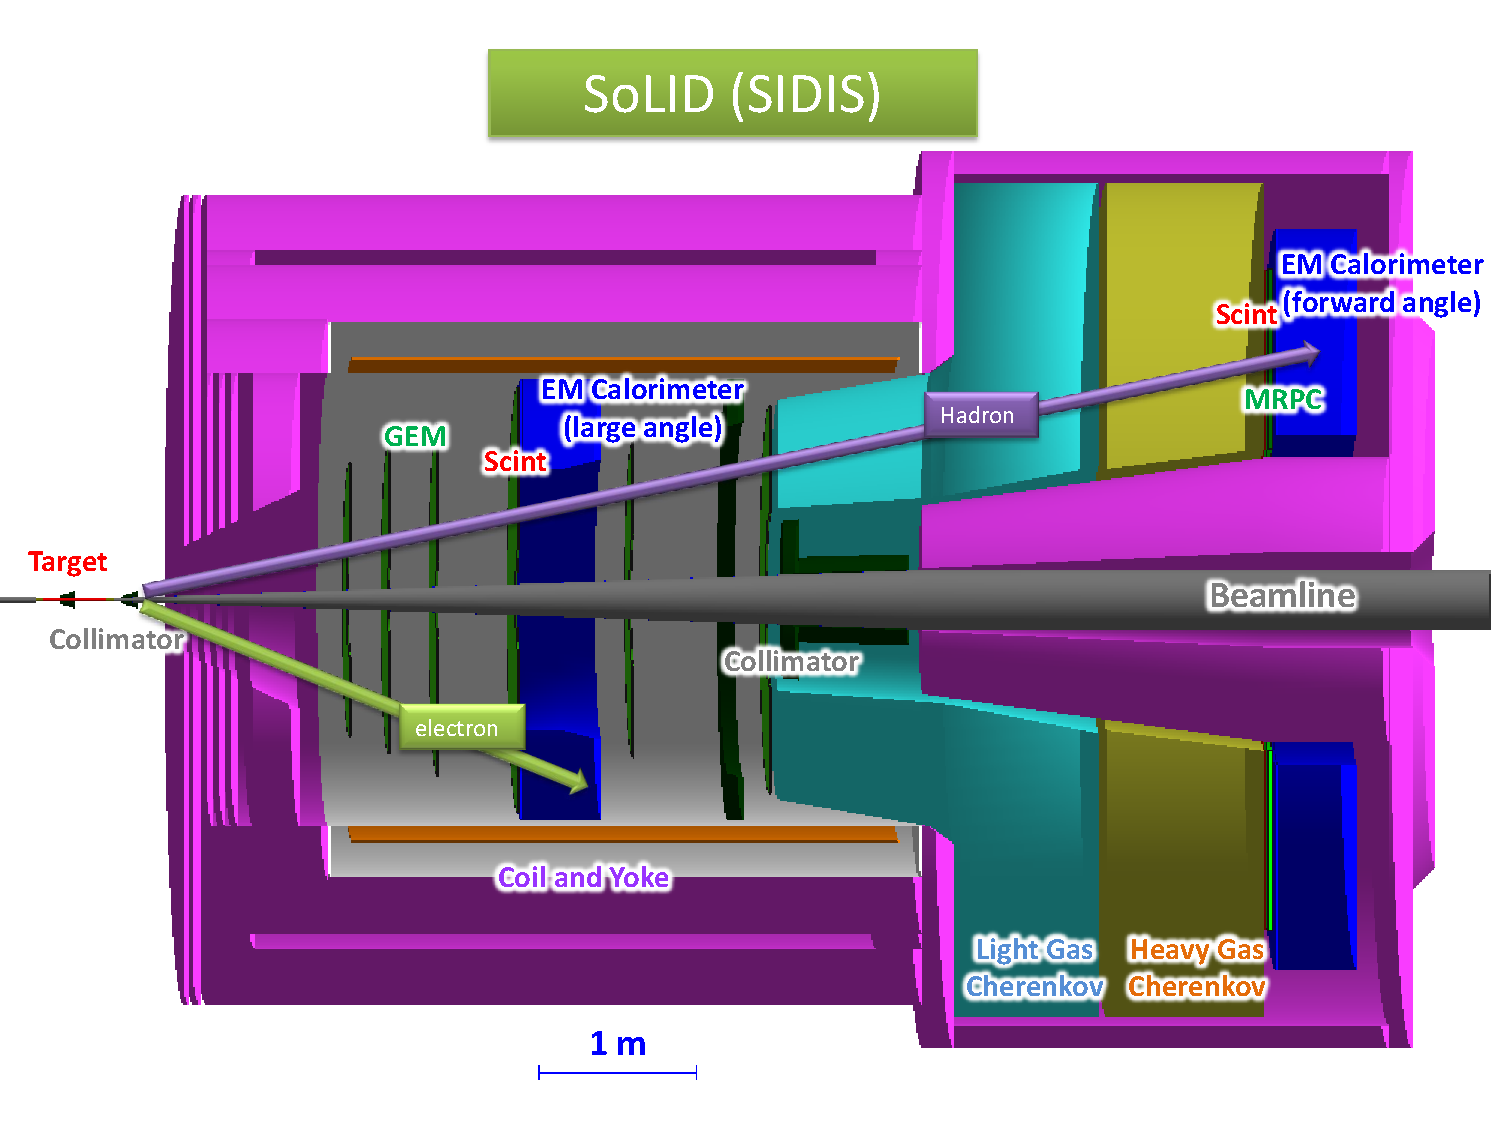
\includegraphics[width=0.6\textwidth]{./figures/SoLID_SIDIS_setup.pdf}
   \caption[The Detector Layout of the SoLID-SIDIS
     configuration]{\footnotesize{The Detector Layout of the SoLID-SIDIS
       configuration. The detector system includes six Gas Electron Multiplier
       (GEM) planes for charged particle tracking, two Scintillator Pad
       Detectors (SPD) followed by two Shashlyk sampling EM Calorimeters (EC)
       for energy measurement and particle identification, a Light Gas
       \v{C}erenkov Detector (LGC) for e-$\pi^{\pm}$ separation, a Heavy Gas
       \v{C}erenkov Detector (HGC) for $\pi^{\pm}$-$K^{\pm}$ separation, as
       well as a Multi-gap Resistive Plate Chamber (MRPC) for timing
       measurement. The first four GEM trackers, the first SPD (i.e. LASPD) and
       EC (i.e. LAEC) form the large-angle detection system for electron
       measurement. The forward-angle detection system, to measure electron and
       hadrons, is composed of all six GEM trackers, LGC, HGC, MRPC, the second
       SPD (i.e. FASPD) and the second EC (FAEC).}}
   \label{solid_sidis}
 \end{center}
\end{figure}

The solenoid magnet for SoLID will be based on the CLEO-II magnet built by
Cornell University. The magnet is 3~meters long with an outer diameter of 3
meters and an inner diameter of 1~meter. The field strength is greater than
1.35~Tesla, with an integrated BDL of 5~Tesla-meters. The fringe field at the
front end after shielding is less than 5~Gauss. In the SIDIS-configuration, the
CLEO-II magnet provides 2$\pi$ acceptance in the azimuthal angle ($\phi$) and
covers polar angle ($\theta$) from 8$^{\circ}$ up to 24$^{\circ}$. The
momentum acceptance is between 0.8 and 7.5~GeV/c for electrons and for hadrons,
the momentum can be lower depending on the trigger efficiency.  The momentum
resolution is about 2\%.

The layout of the SoLID detectors in the SIDIS-configuration is shown in
Fig.~\ref{solid_sidis}. The detector system is divided into two regions for the
forward-angle (FA) detection and the large-angle (LA) detection. Six tracking
chambers based on Gas Electron Multipliers (GEM) will be used for charged
particle tracking in the forward-angle region, and the first four of them will
be shared by the large-angle
region. In each region, a Shashlyk-type sampling EM calorimeter (LAEC or
FAEC) will measure the particle energy and identify electrons from hadrons. A
scintillator-pad detector (LASPD and FASPD) will be installed in front of each
EC to reject photons and provide timing information. The forward-angle
detectors will detect both the electrons and hadrons (mainly $\pi^{\pm}$). A
light-gas \v{C}erenkov detector (LGC) and a heavy-gas \v{C}erenkov detector
(HGC) will perform the $e/\pi^{\pm}$ and $\pi^{\pm}/K^{\pm}$ separation,
respectively. The Multi-gas Resistive Plate Chamber (MRPC) will provide a
precise timing measurement and serve as a backup of the FASPD on photon
rejection. A more detailed discussion of the design, simulation, prototype-test
of each detector is given in the SoLID preliminary conceptual design report
(pCDR)~\cite{solid_pcdr}.

Table~\ref{table:key_par_sidis_dvcs} summarizes the key parameters of the
detector system in the SIDIS configuration for both the SIDIS and DEMP
measurements.
\begin{table}\centering
\begin{tabular}{|c|c|c|c|c|}
\hline
Experiments                & SIDIS                    & DEMP  \\\hline
Reaction channel           & $\vec{n}(e,e'\pi^{\pm})X$ & $\vec{n}(e,e'\pi^{-}p)$	\\\hline
Target                     & $^3$He                   &same 	\\\hline
Unpolarized luminosity     & $\sim10^{37}$ cm$^{-2}$s$^{-1}$ per nucleon & same	\\\hline 
Momentum coverage          & 0.8-7.5 (GeV/c) for  $e^-$,$\pi^{\pm}$           &same 	\\
          										&   & 0.3~1.2 (GeV/c) for protons	\\\hline
Momentum resolution        & $\sim$2\%                & same\\\hline
Azimuthal angle coverage   & 0$^{\circ}$ ~360$^{\circ}$ & same	\\\hline
Azimuthal angle resolution & 5 mr                     & same	\\\hline
Polar angle coverage       & 8$^{\circ}$-24$^{\circ}$ for $e$ &  same \\
       & 8$^{\circ}$-14.8$^{\circ}$ for $\pi^{\pm}$  &  same 	\\
                           &                          & 8$^{\circ}$-24
                                                        $^{\circ}$ for $p$ in SoLID\\
                           &                          & 24$^{\circ}$-50$^{\circ}$ for $p$ with recoil detector         \\\hline
Polar angle resolution     & 0.6 mr                   & same	\\\hline
Target Vertex resolution   & 0.5~cm                   & same \\\hline
 Energy resolution on ECs  & 5\%$\sim$10\%            & same   \\\hline
Trigger type               & Double Coincidence $e^-+\pi^{\pm}$ & same (online)\\
              &  & Triple Coincidence $e^-+\pi^{-}+p$ (offline)\\\hline

Expected DAQ rates         &  $<$100 kHz              &  same (online)\\\hline

Main Backgrounds           & $\mathrm{^{3}He}$(e,e'K$^\pm$/$\pi^{0}$)X            &$\mathrm{^{3}He}$(e,e'$\pi^{\pm}$/K$^\pm$)X  \\
                           &   Accidental Coincidence & Accidental Coincidence	\\\hline
Key requirements           &  Radiation hardness      & Proton Detection	\\
                           &  Kaon Rejection          & Exclusivity	\\
                           &  DAQ                     &    Timing Resolution   \\
                        \hline
\end{tabular}
\caption{\footnotesize{Summary of Key Parameters for DEMP Measurement compared
    with SIDIS Experiments.}}\label{table:program_summary}
\label{table:key_par_sidis_dvcs}
\end{table} 

%\newpage
\subsection{Recoil Proton Identification}

\begin{figure}[!ht]
 \begin{center}
  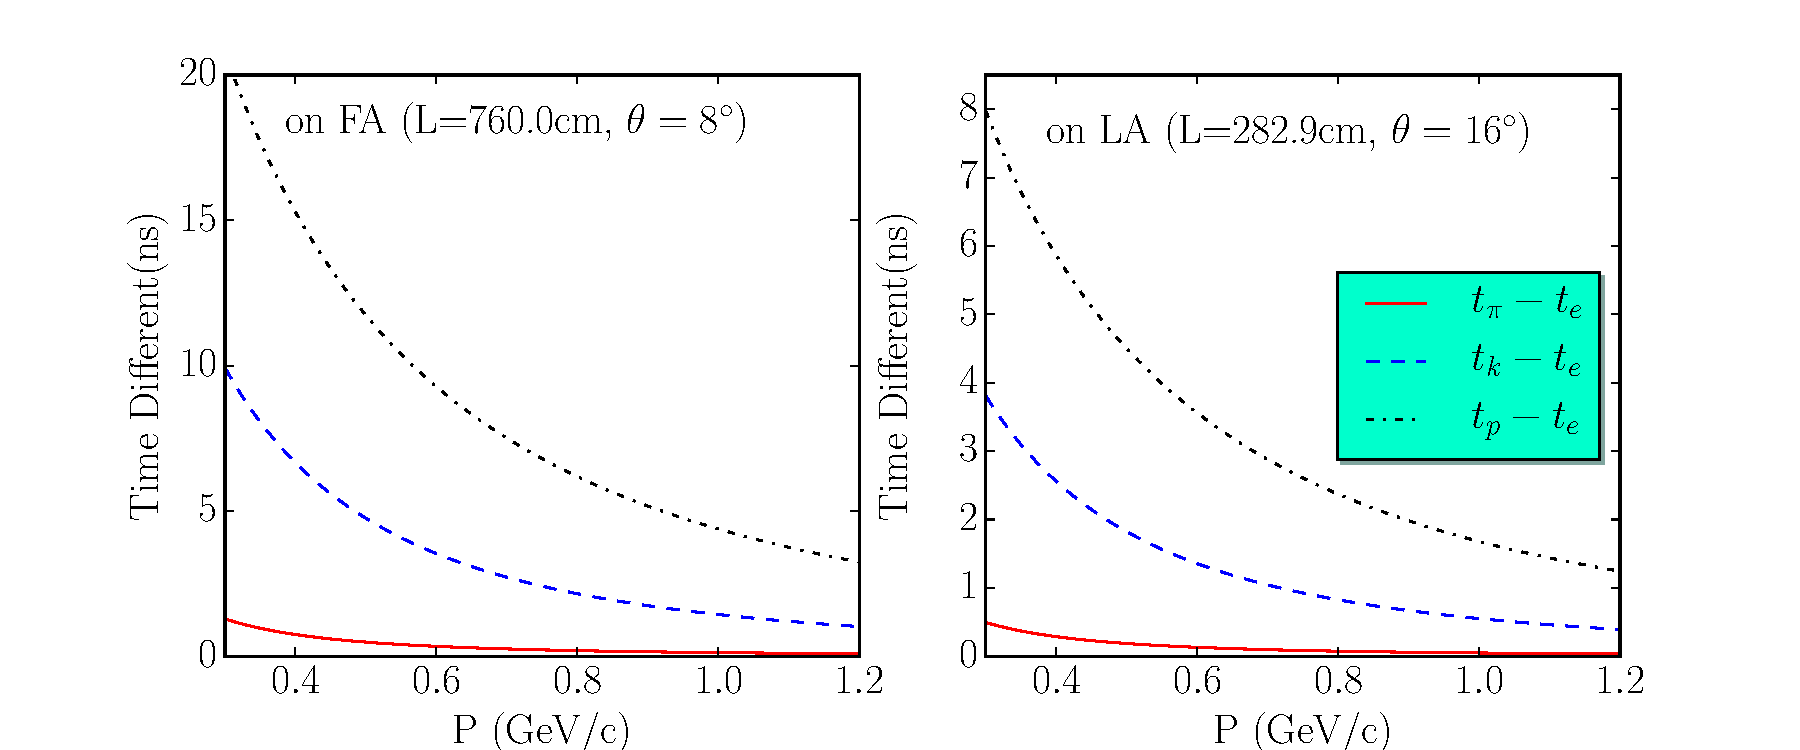
\includegraphics[width=0.8\textwidth]{./figures/time_diff.pdf}
   \caption[Time-of-time]{\footnotesize{The time differences (in $ns$) between
       electrons and other charged particles, i.e. pions (red solid line),
       kaons (blue dashed line) and proton (black dash-dotted line), and their
       distributions as functions of particles' momentum at three different
       timing detectors, including the forward-angle (FA) MRPC and the large-angle
       (LA) SPD.}}
   \label{tof_diff}
 \end{center}
\end{figure}

The cleanest way to identify the DEMP events is to detect all particles in the
final state. The SoLID-SIDIS detector system has the capability of measuring
electrons and pions, while protons can be isolated from other charged particles
by using the time-of-flight (TOF) information. The TOF is provided by the timing
detectors, including the MRPC and FASPD at the forward-angle detection region,
and the LASPD at the large-angle detection region. 

We examined the requirement of the timing resolution on these detectors by
looking at the time difference between electrons and other heavier charged
particles when they reach these detectors with the same momentum and flight
path. As shown in the next section, the good protons from the DEMP reaction
carry momenta from 0.3~GeV/c up to 1.2~GeV/c with angles from
$0^{\circ}$ to $50^{\circ}$. The FA-MRPC covers angles from
$8^{\circ}$ to $14.8^{\circ}$, and the angular range of the LASPD is from
$16^{\circ}$ to $24^{\circ}$.  Hence we simulated
events of electrons, pions, kaons and protons with the momentum from
0.3~GeV/c up to 1.2~GeV/c, and calculated the time when they reach three
detectors with linear trajectories and at fixed angles.

The results are shown in Fig.~\ref{tof_diff}. To clearly identify two types of
charged particles with the same momentum, we normally require the timing
difference between two particles to be larger than 5 times of the overall
timing resolution, while the SoLID timing detectors can reach the resolution
in the range of 150~ps down to 50~ps.  At the FA-MRPC, which is more than 7
meters from the target, protons come 3~ns later than kaons, even at the
highest momenta in the DEMP reaction. Hence, protons will be easily distinguished
from other lighter particles.  At the LA-SPD, which is about 3 meters away from
the target, the time difference between protons and kaons is still more than
1~ns, which doesn't demand precise timing resolution.

In general, the misidentified events can be mostly removed by cutting on the
reconstructed missing quantities, e.g. angles, momenta and masses. The residual
background will also be largely suppressed in the target-spin asymmetry
extraction.

\subsection{Trigger Design}

In E12-10-006, the online production trigger will be the double-coincidence of
the scattered electrons and hadrons. One will use the particle identification
detectors, such as LGC, HGC and ECs, during the offline analysis to select
$\pi^{\pm}$ out from other hadrons. The DEMP events will be identified with the
triple-coincidence of the scattered electron, $\pi^{-}$ and proton, while the
proton identification has been discussed above. We will use the same online
trigger as the SIDIS one, and hence the new experiment will share the same
data-set as E12-10-006. The actual design of the SIDIS triggers will be far
more complicated, and the detailed discussion of the trigger and DAQ designs is
given in the SoLID pCDR~\cite{solid_pcdr}.
